% fig1_framework.pdf — SEAL/TGRS architecture overview
% Stage A: frozen COCO-init Mask2Former-R50 base (unchanged)
% Stage B: training-free recovery stack  soup -> wide 8-view TTA -> consensus fusion
% Optional: boundary-patch refinement (dashed)
% Numbers: E:/SAR/seal/docs/ALL_TABLES.md (T1). Compile: pdflatex (standalone).
% This MiKTeX lacks grfext.sty (dependency of epstopdf-base, auto-loaded by
% graphics.cfg under pdflatex). We need no EPS conversion, so mark it loaded:
\expandafter\def\csname ver@epstopdf-base.sty\endcsname{2020/01/24}
\documentclass[tikz,border=3pt]{standalone}
\usepackage{mathptmx}% Times text+math (newtx not installed in this MiKTeX)
\usepackage[T1]{fontenc}
\usepackage{amssymb}% \mathbb
\usetikzlibrary{positioning,arrows.meta,fit,backgrounds,calc}

\definecolor{cblue}{HTML}{1f77b4}
\definecolor{corange}{HTML}{ff7f0e}
\definecolor{cgray}{HTML}{7f7f7f}
\definecolor{fillA}{HTML}{eef3f8}
\definecolor{fillB}{HTML}{fef3e8}

\begin{document}
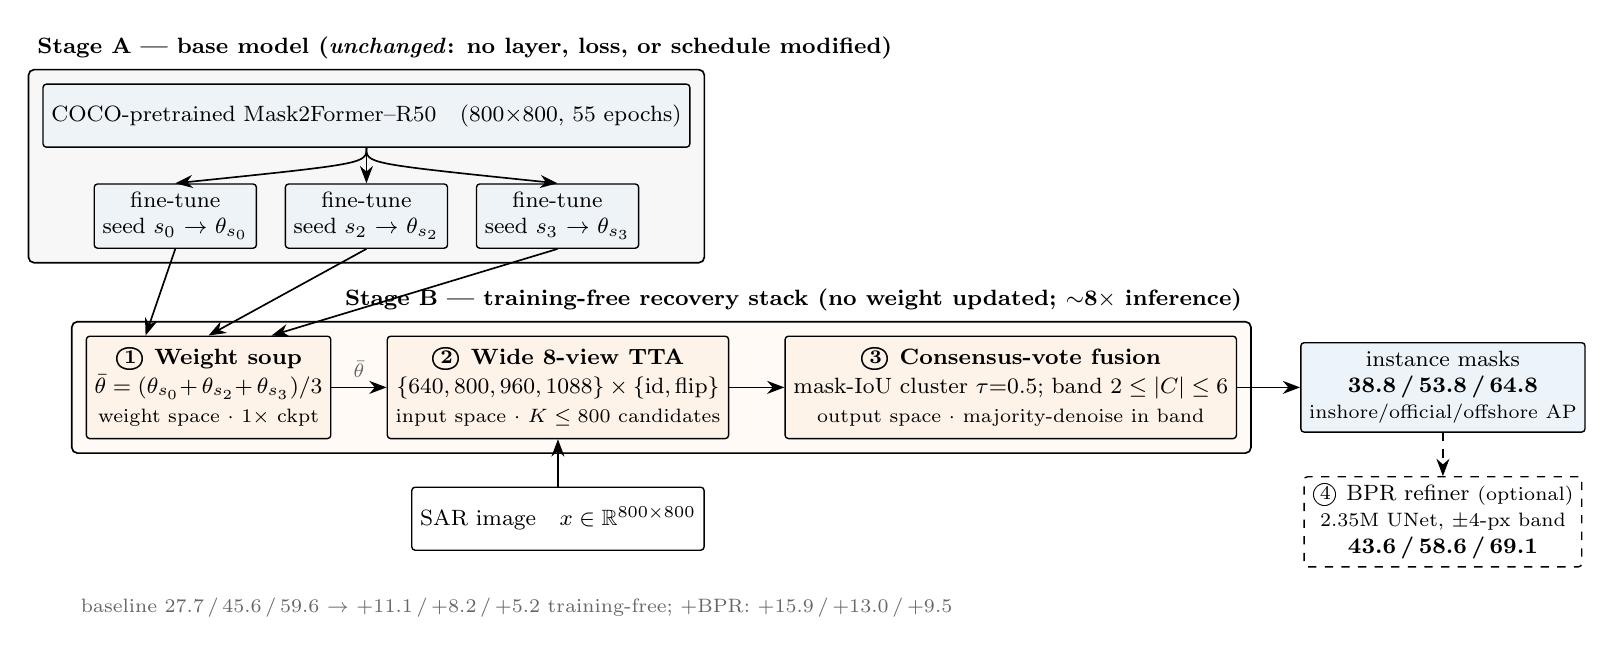
\begin{tikzpicture}[
  font=\footnotesize,
  >={Stealth[length=2.2mm]},
  node distance=4mm and 6mm,
  box/.style={draw=black, line width=0.5pt, rounded corners=1.2pt, align=center,
              inner sep=3pt, minimum height=8mm},
  ckpt/.style={box, fill=fillA, minimum width=17mm},
  op/.style={box, fill=fillB, minimum width=30mm, minimum height=13mm},
  io/.style={box, fill=white, minimum width=17mm},
  stage/.style={draw, line width=0.6pt, rounded corners=2pt, inner sep=5pt},
  lbl/.style={font=\footnotesize\bfseries},
  sub/.style={font=\scriptsize, text=black!60},
  arr/.style={->, line width=0.6pt},
]

% ---------------- Stage A: frozen base ----------------
\node[ckpt] (s0) {fine-tune\\seed $s_0$ $\to$ $\theta_{s_0}$};
\node[ckpt, right=3.5mm of s0] (s2) {fine-tune\\seed $s_2$ $\to$ $\theta_{s_2}$};
\node[ckpt, right=3.5mm of s2] (s3) {fine-tune\\seed $s_3$ $\to$ $\theta_{s_3}$};
\node[box, fill=fillA, above=4.5mm of s2, minimum width=56mm]
  (base) {COCO-pretrained Mask2Former--R50\quad(800$\times$800, 55 epochs)};
\draw[arr] (base.south) -- (s2.north);
\draw[arr] (base.south) .. controls +(0,-2mm) .. (s0.north);
\draw[arr] (base.south) .. controls +(0,-2mm) .. (s3.north);

\begin{scope}[on background layer]
\node[stage, fit=(base)(s0)(s3), fill=black!3] (stageA) {};
\end{scope}
\node[lbl, anchor=south west] at (stageA.north west)
  {Stage A --- base model (\emph{unchanged}: no layer, loss, or schedule modified)};

% ---------------- Stage B: training-free recovery stack ----------------
\node[op, below=11mm of s0.south west, anchor=north west, xshift=-1mm]
  (soup) {\textbf{\textcircled{\scriptsize 1} Weight soup}\\[1pt]
          $\bar\theta=(\theta_{s_0}{+}\,\theta_{s_2}{+}\,\theta_{s_3})/3$\\[1pt]
          {\scriptsize weight space $\cdot$ 1$\times$ ckpt}};
\node[op, right=7mm of soup]
  (tta) {\textbf{\textcircled{\scriptsize 2} Wide 8-view TTA}\\[1pt]
         $\{640,800,960,1088\}\times\{\mathrm{id},\mathrm{flip}\}$\\[1pt]
         {\scriptsize input space $\cdot$ $K\le800$ candidates}};
\node[op, right=7mm of tta]
  (cons) {\textbf{\textcircled{\scriptsize 3} Consensus-vote fusion}\\[1pt]
          mask-IoU cluster $\tau{=}0.5$;\ band $2\le|C|\le6$\\[1pt]
          {\scriptsize output space $\cdot$ majority-denoise in band}};
\draw[arr] (soup) -- node[above, sub] {$\bar\theta$} (tta);
\draw[arr] (tta) -- (cons);

% checkpoints feed the soup (straight, order-preserving: no crossings)
\draw[arr] (s0.south) -- ($(soup.north)+(-8mm,0)$);
\draw[arr] (s2.south) -- (soup.north);
\draw[arr] (s3.south) -- ($(soup.north)+(8mm,0)$);

\begin{scope}[on background layer]
\node[stage, fit=(soup)(tta)(cons), fill=corange!4] (stageB) {};
\end{scope}
\node[lbl, anchor=south east] at (stageB.north east)
  {Stage B --- training-free recovery stack (no weight updated; $\sim$8$\times$ inference)};

% ---------------- input / output ----------------
\node[io, below=6mm of tta] (img) {SAR image\quad$x\in\mathbb{R}^{800\times800}$};
\draw[arr] (img.north) -- (tta.south);

\node[io, right=8mm of cons, fill=cblue!8, minimum width=24mm]
  (out) {instance masks\\\textbf{38.8\,/\,53.8\,/\,64.8}\\{\scriptsize inshore/official/offshore AP}};
\draw[arr] (cons) -- (out);

% ---------------- optional BPR (dashed) ----------------
\node[box, dashed, below=5.5mm of out, fill=white, minimum width=24mm]
  (bpr) {\textcircled{\scriptsize 4} BPR refiner {\scriptsize(optional)}\\
         {\scriptsize 2.35M UNet, $\pm$4-px band}\\
         \textbf{43.6\,/\,58.6\,/\,69.1}};
\draw[arr, dashed] (out) -- (bpr);

% baseline note under Stage B (below the input node to avoid overlap)
\node[sub, anchor=north west] at ($(stageB.south west)+(0,-17mm)$)
  {baseline 27.7\,/\,45.6\,/\,59.6 $\to$ +11.1\,/\,+8.2\,/\,+5.2 training-free; +BPR: +15.9\,/\,+13.0\,/\,+9.5};

\end{tikzpicture}
\end{document}
